\newpage
\section{Исследовательская часть}
\subsection{Обоснование области исследования}
\textit{\textbf{Оптический поток (Optical flow)}} – технология, использующаяся в различных областях компьютерного зранеия для определения сдвигов, сегментации, выделения объектов, компрессии видео и прочего. В специализированной литературе и глобальной сети Internet много вводных статей в эту технологию, в которых рассмотрены основные шаги для реализиции оптического потока в своих проектах. Однако, при попытке реализовать оптический поток самостоятельно на основе полученной информации, такие реализации  работают очень плохо и сбоят при определении сдвигов уже порядка 1-2 пикселей.

В таких случаях следует обратиться к готовым реализациям этих методов. В настоящий момент наиболее развитой библиотекой компьютерного зрения является OpenCV\cite{wikiOpenCV}. Но в этой библиотеке реализовано множество способов вычисления оптического потока, у каждого из которых неколько параметров, которые как-то оказывают влияние на качество и сокрость работы алгоритмов. 

В данной работе оптический поток играет ключевую роль, а время его вычисления занимает более половины времени работы всей системы. В связи с чем, в исследовательской части будут рассмотрены реализованные в OpenCV методы вычисления оптического потока, исследованно влияние их параметров на скорость работы алгоритмов, а так же оценено время работы каждого из методов при разных входных данных, приближенных к условиям работы разрабатываемой системы.

\subsection{Описание исследуемых методов}
\subsubsection{метод Лукаса-Канаде}
Метод Лукаса-Канаде является стандартным подходом к вычислению оптического потока, так как обладает достаточно низкой ресурсоемкостью и временем выполнения. В основном это достигается за счет вычисления не плотного оптического потока, а выборочного, для определенных точек изображения. Подробно этот алгоритм был рассмотрен в пункте \ref{label:lucas-kanade-math}. 

\subsubsection{Horn–Schunck}
Метод Horn–Schunck носит несколько более глобальный характер, чем метод Лукаса-Канаде. Он опирается на предположение о том, что на всем изображении оптический поток будет достаточно гладким.

Этот алгоритм был реализован в первых версиях OpenCV, но в последствии от него отказались по причине его плохой приспособленности к реальным видеопотокам. Данный метод упомянут только для ознакомления, в дальнейшем он не будет рассматриваться. 

\subsubsection{Farneback}
В данном методе предлагается аппроксимировать изменение интенсивности в окрестности с помощью квадратичной формы: $I = xAx + bx + c$ с симметричной матрицей $A$ (по сути, рассматривая разложение по Тейлору до первого члена, мы брали линейную аппроксимацию I = bx + c. используя указанное разложение мы увеличиваем точность апроксимации.)
Если изображение сдвинулось в пределах этой окрестности, то 
$I_2 (x) = I_1 (x-d)$, подствавив в квадратичное разложение и раскрываем скобки, получаем:

$$ A_2 = A_1 $$
$$ b_2 = b_1 - 2A_1d $$
$$ c_2 = d^TA_1d - b_1^Td + c_1 $$
Вычисляя значения $A, b, c$ на обеих картинках, полчим избыточную систему относительно d. Более того, приближенное значение $d$ можно получить из второго уравнения: 
$$ d = -\frac{1}{2} \cdot A^{-1} \ cdot (b2 - b_1) $$

\subsubsection{SimpleFlow}
В основе метода SimpleFlow лежит следующая идея: если все равно нет возможности определять сдвиг больше чем размер окна, по которому мы искали производные, то можно просто в окне найти наиболее похожую точку. А для разрешения неоднозначностей и для компенсации шумов учитывать, что поток непрерывный и в окрестности данной точки все точки имеют почти одинаковый сдвиг. Возникающие трудности с размером окна возможно решить за счет multi-scaling'а\footnote{итеративное вычисление оптичесокго потока для уменьшенных изображений с целью определения больших сдвигов.}.

\subsubsection{Dual TV L1}
В ходе написания данной работы, 25 апреля 2014 года, была выпущена новая версия OpenCV 2.4.9, в которой был реализован еще одни метод вычисления оптического потока - Dual TV L1. 
К сожалению к этому моменту эксперимент был завершен и исследование еще и этого метода не представлялось возможным. 

\subsection{Проведение эксперимента}

Целью эксперимента было выявление зависимостей времени вычисления оптического потока разными методами от размера кадров и различных параметров этих методов.

\subsubsection{Методика проведения эксперимента}
Эксперимент проводился следующим образом.
Для анализа производтельности каждым методом анализировался видеофайл длительностью 10 секунд и с частотой кадров - 30 кадров/сек. Итого оптический поток был высчитан для 299 кадров (для первого кадра не вычисяляется). Размер кадра изменялся от 160*90 до 1280*720 пикселей с увеличением кадра в 2 раза на каждом тесте.

\subsubsection{Исходный код программы}
Для проведения эксперимента была написана программа на языке Java с использовании библиотеки JavaOpenCV. 

\begin{verbatim}
     1	public Mat onCameraFrame(CvCameraViewFrame inputFram
e) {
     2	   
     3	    mGray = inputFrame.gray();
     4	    Mat resizeImg = new Mat();
     5	
     6	    if (mPrevGray != null && !mPrevGray.empty()) {
     7	       
     8	        MatOfKeyPoint mKeyPoint = new MatOfKeyPoint(
);
     9	        FeatureDetector.create(FeatureDetector.HARRI
S).detect(mPrevGray, mKeyPoint);
    10	
    11	        ArrayList<Point> temp = new ArrayList<Point>
();
    12	        List<KeyPoint> keyPointsList = mKeyPoint.toL
ist();
    13	        for (int i = 0; i<keyPointsList.size(); i++)
    14	        {
    15	            temp.add(keyPointsList.get(i).pt);
    16	        }
    17	        MatOfPoint2f needs = new MatOfPoint2f();
    18	        needs.fromList(temp);
    19	        MatOfPoint2f result = new MatOfPoint2f();
    20	        MatOfByte status = new MatOfByte();
    21	        MatOfFloat err = new MatOfFloat();
    22	
    23	        calcOpticalFlowPyrLK(mPrevGray, mGray, needs
, result, status, err);
    24	
    25	    }
    26	
    27	    mPrevGray = mGray;
    28	    count++;
    29	
    30	return mGray;
    31	}

\end{verbatim}

\subsubsection{Тестовый стенд}
Сначала тестирвоание проводилось на настольном персональном коипьютере со следуюшими характеристиками:

\begin{itemize}
\item процессор Intel Core i7 с тактовой частотой 3100МГц; 
\item 4ГБ оперативной памяти.
\end{itemize}

Однако при такой конфигурации оборудования отличия во времени выполнения на разных размерах кадра были незначительными, поэтому эксперимент был проведен на смартфоне LG Nexus 4 со следующими характериситками:
\begin{itemize}
\item процессор Intel Core i7 с тактовой частотой 1500МГц;
\item 2ГБ оперативной памяти.
\end{itemize}

\subsubsection{Результаты эксперимента}
Отпический поток высчитывался 3-мя методами: SimpleFlow, Farneback и Lucas-Kanade. Все эти три метода реализованы в библиотеке компьютерного зрения OpenCV и вначале вызывались со стандартными параметрами. Замерялось время вычисления ОП для всей видеопоследовательности. Результаты эксперимента представлены на рисунке~\ref{pic:compareMethods}.

\begin{figure}[!htb]
\center{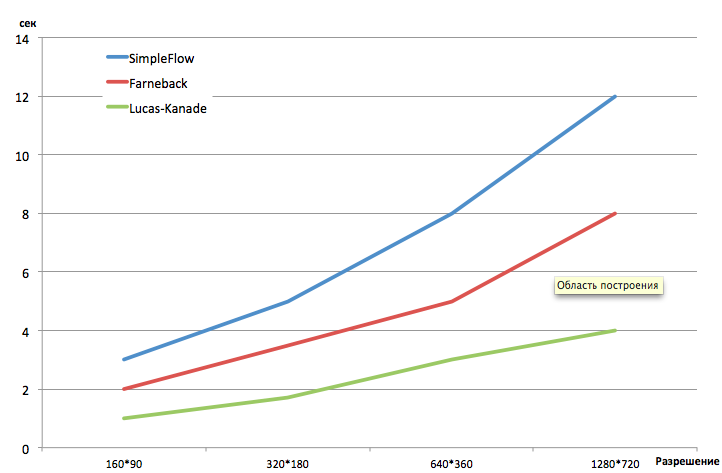
\includegraphics[width=0.8\linewidth]{pics/compareMethods.png}}
\caption{Сравнение времени выполнения методов вычисления оптического потока}
\label{pic:compareMethods}
\end{figure}

Из графика видно, что методо Лукаса-Канаде является самым быстрым, что обусловлено тем, что этим методом вычисляется лишь выборочный поток, а не плотный. 

Тем не менее, методы обладают рядом параметров, которые могут позволить увеличить их производительность. В связи с этим были проведено исследование их влияния на общее время вычисления оптического потока. 

\paragraph{Farneback}
Согласно документации OpenCV метод Farneback имеет следующие параметры.
\begin{itemize}
\item \textit{prev} – первое изображение.
\item \textit{next} – второе изображение.
\item \textit{flow} – вычисленный оптический поток в виде векторов. 
\item \textit{pyr--scale} – параметр, характеризующий коэф. уменьшения изображений при построении пирамиды. Стандартное значение - 0,5.
\item \textit{levels} – число уровне в пирамиде. Стандартное значение - 3.
\item \textit{winsize} – средний размер окна. Стандартное значение - 15.
\item \textit{iterations} – число итераций на каждом уровне пирамиды. Стандартное значение - 3.
\item \textit{poly--n} – число пикселей, используемых для идентификации ключевых точек. Стандартное значение - 5.
\item \textit{poly--sigma} – стандартное отклонение Гаусса, используемое для сглаживания производных. Стандартное значение - 1,1.
\end{itemize}

Очевидно, что первые три параметра изменять нельзя, кроме размера самих кадров, что мы и так делаем. 
На рисунке~\ref{pic:3FB_params} показано влияние других параметров на время вычисления оптического потока. 

\begin{figure}[!Htb]
\begin{minipage}[h]{0.47\linewidth}
\center{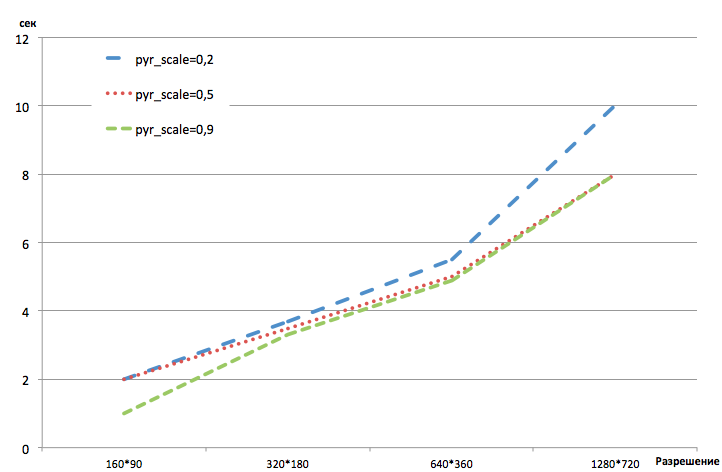
\includegraphics[width=1\linewidth]{pics/3FB_pyrscale.png}} a) \\
\end{minipage}
\hfill
\begin{minipage}[h]{0.47\linewidth}
\center{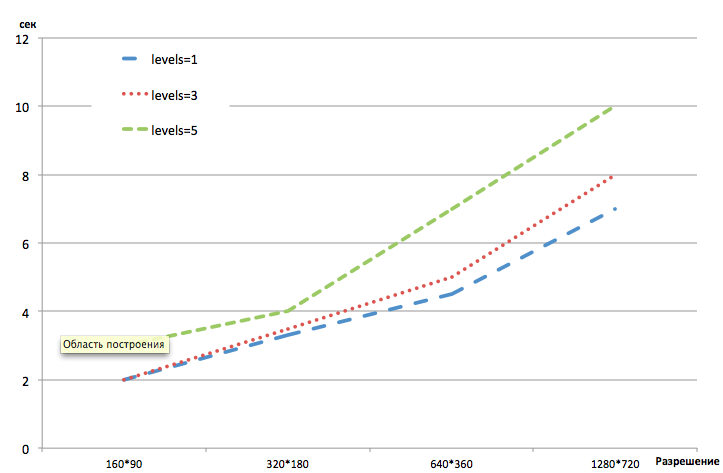
\includegraphics[width=1\linewidth]{pics/3FB_levels.png}} б)\\
\end{minipage}
\vfill
\begin{minipage}[h]{0.47\linewidth}
\center{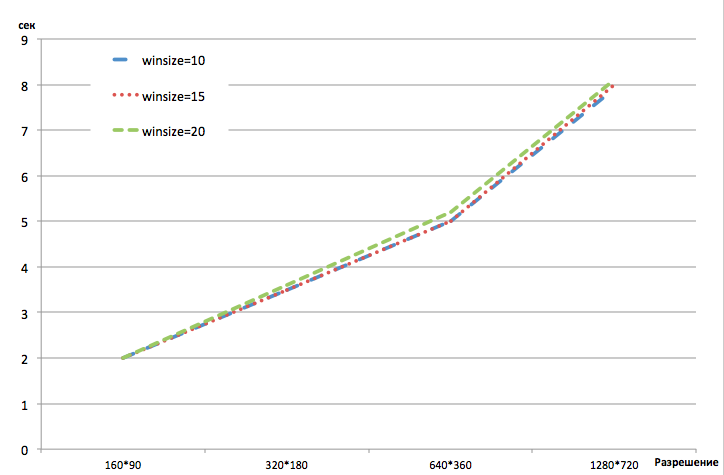
\includegraphics[width=1\linewidth]{pics/3FB_winsize.png}} в) \\
\end{minipage}
\hfill
\begin{minipage}[h]{0.47\linewidth}
\center{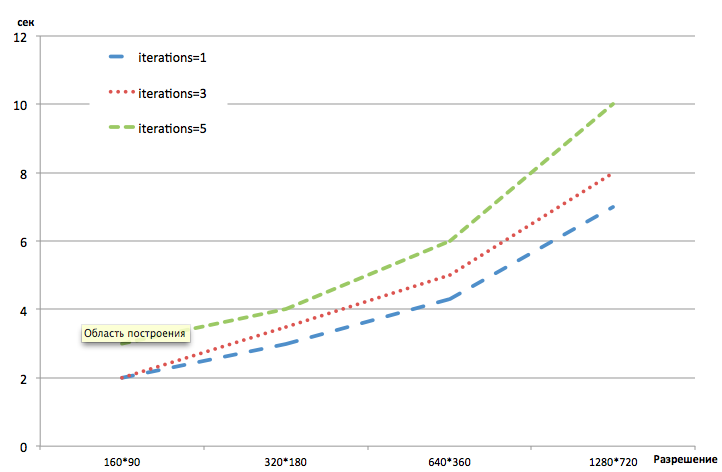
\includegraphics[width=1\linewidth]{pics/3FB_interation.png}} г) \\
\end{minipage}

\begin{center}
	\begin{minipage}[h]{0.47\linewidth}
	\center{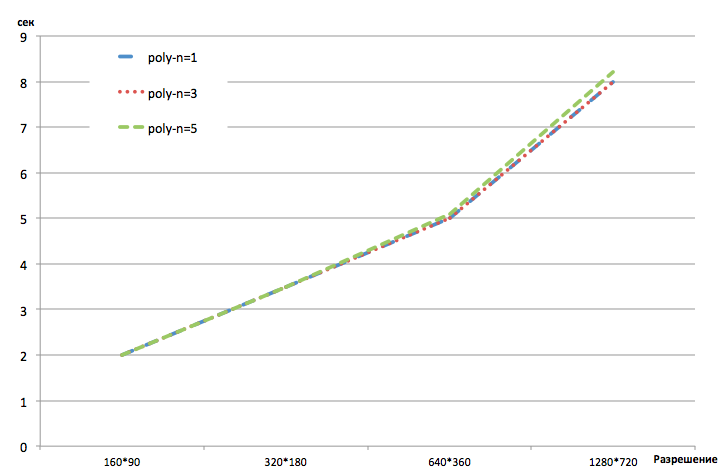
\includegraphics[width=1\linewidth]{pics/3FB_polyn.png}} д) \\
	\end{minipage}
\end{center}
\caption{Влияние значения параметров на время работы алгоритма: а)pyr--scale; б)  levels; в) winsize ; г) interation; д) poly--n}
\label{pic:3FB_params}
\end{figure}

Из графиков видно, что снизить время выполнения можно путем уменьшения уровней в пирамиде, однако такой подход снижает точность вычисления оптического потока. К сожалению, выразить точность вычисления в измеримой величине сложно. Такая же ситуация с числом итераций interation - снижение их числа снижает время выполнения, но качество вычисления потока снижается. 

\paragraph{SimpleFlow}
Согласно документации OpenCV метод SimpleFlow имеет следующие параметры.
\begin{itemize}
\item \textit{prev} – первое изображение.
\item \textit{next} – второе изображение.
\item \textit{flow} – вычисленный оптический поток в виде векторов. 
\item \textit{layers} – число уровней при построении пирамиды. Стандартное значение - 3.
\item \textit{averaging--block--size} – размер окна, по которому происходит поиск пикселей. Стандартное значение - 2. 
\item \textit{max--flow} – максимальный сдвиг для всех уровней пирамиды. Стандартное значение - 4.
\end{itemize}

Так же очевидно, что первые три параметра являются опорными и не подлежат изменению в рамках эксперимента. Влияние последних трех параметров на время вычисления оптического потока методом SimpleFlow показано на рисунке~\ref{pic:3SF_params}
\begin{figure}[!Htb]
\begin{minipage}[h]{0.47\linewidth}
\center{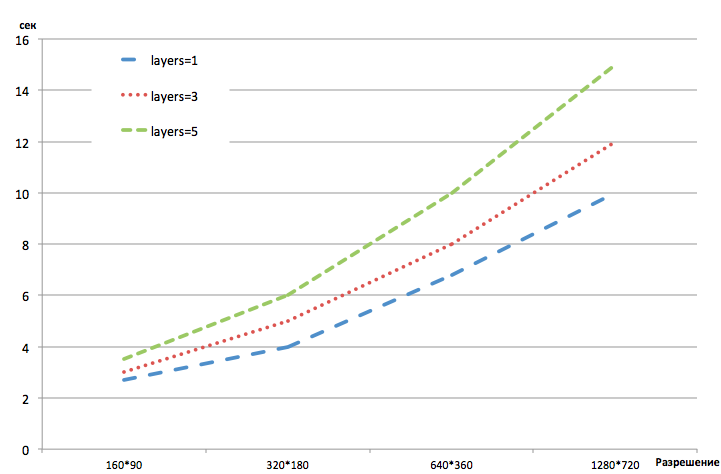
\includegraphics[width=1\linewidth]{pics/3SF_layers.png}} a) \\
\end{minipage}
\hfill
\begin{minipage}[h]{0.47\linewidth}
\center{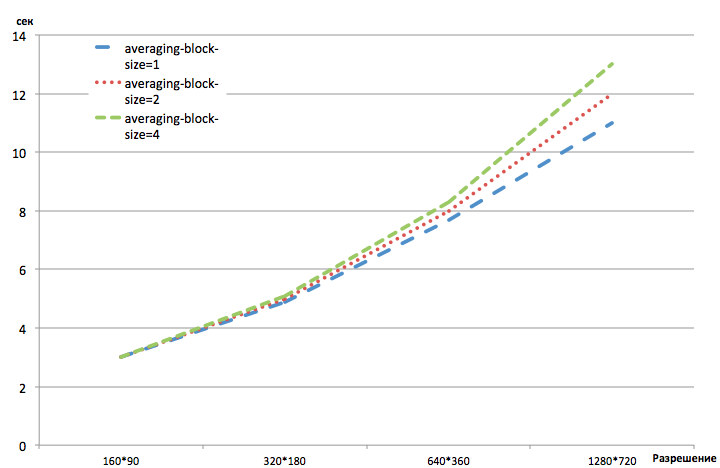
\includegraphics[width=1\linewidth]{pics/3SF_avgBlockSize.png}} б)\\
\end{minipage}
\vfill
\begin{center}
	\begin{minipage}[h]{0.47\linewidth}
	\center{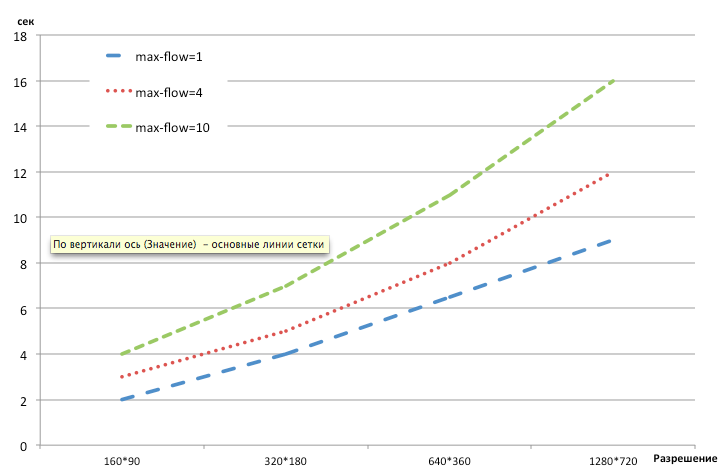
\includegraphics[width=1\linewidth]{pics/3SF_maxflow.png}} в) \\
	\end{minipage}
\end{center}
\caption{Влияние значения параметров на время работы алгоритма: а)layers; б)  averaging--block--size; в) max--flow;}
\label{pic:3SF_params}
\end{figure}

Из графиков видно, что нибольшее влияние оказывает параметр max--flow, но так как он ограничивает значения максимального оптического потока, то для нахождения всех возможных сдвигов в ходе быстрого движения в кадре, этот параметр должен быть близок к  $max (высота кадра, ширина кадра) $. Таким образом, уменьшение данного параметра до 1, снижает время вычисления, но делает работу алгоритма бессмыленной, так как сдвиги более чем на 1 пиксель не будут найдены.  


\subsection{Выводы к исследовательской части}
В ходе проведения экспериментов было установлено следующее:
\begin{itemize}
\item Алгоритм Лукаса-Канаде работает быстрее алгоритмов SimpleFlow и Farneback. Причем разница более заметна при больших разренениях кадра. 
\item Алгоритмы SimpleFlow и Farneback имееют несколько параметров, оказывающих влияние на время их выполнения, однако при уменьшении времени выполнения снижается и качество вычисления результирующего оптического потока. 
\item При необходимости высчитывать оптический поток в реальных условиях, самым приемлемым являемя алгоритм Лукаса-Канаде, которые показывает нименьшее время выполнения при приемлемом качестве. Такое преимущество возникает из-за вычисления не плотного, а выборочного оптического потока. 
\end{itemize}